\chapter{Kameramodelle}
\label{sec:CameraModels}



Also Kameramodell wird der rechnerische Prozess genannte, welcher Objekte aus dem 3D-Raum auf ein ein 2D-Bild projiziert und andersherum\cite{CamerModels.,HZ}. Das einfachste Kameramodell ist das Lochkameramodell. Die Reduktion einer Dreidimensionalen Welt in ein Zweidimensionales Bild, ist ein Prozess bei welchem durch eine, in den meisten Fällen angewandte, Zentralprojektion eine Dimension verloren geht\cite{HZ}. Bei einer Zentralprojektion wird ein Strahl von einem Punkt im 3D-Raum durch das Projektionszentrum der Kamera gezogen. Das Projektionszentrum der Kamera beschreibt den Punkt in der Kamera an welchem sich alle Strahlen treffen. Ein Strahl der durch einen Punkt im 3D-Raum und durch das Projektionszentrum einer Kamera geht, schneidet eine Ebene, welche im weiteren Verlauf als Bildebene bezeichnet wird. Der Schnittpunkt des Strahls mit der Bildebene wird Bildpunkt genannt\cite{CamerModels.,HZ}.\\


(GRAFIK PROJEKTION ANFERTIGEN SIEHE ABB 1 AUF NOTIZZETTEL)\\

\subsection{Lochkameramodell}

Das Kameramodell, auf welchem diese Arbeit aufbaut, ist das sogenannten Lochkameramodel. Das Lochkameramodell ist eines der am simpelsten aufgebauten Kameramodelle und wird standardmäßig zur Beschreibung optischer Kameras verwendet. Das Modell beruht ausschließlich auf der geometrischen Optik und vernachlässigt physikalische Effekte wie Beugung oder die Auswirkung der Linse\cite{heipke}. Das Lochkameramodell beinhaltet ein Projektionszentrum $C$, welches auch gleichzeitig das Kamerazentrum bildet. Die Kamera an sich wird im Lochkameramodell als Punkt angegeben und ist meist gleichbedeutend mit dem Punkt $C$. $C$ besitzt ein eigenes Dreidimensionales Koordinatensystem. Das Kamerakoordinatensystem und alle weiteren Koordinatensysteme, die noch eingeführt werden, dienen dazu die Position eines Punktes innerhalb ihres geometrischen eindeutig zu bezeichnen. Das Kamerakoordinatensystem hat seinen Ursprung im Projektionszentrum $C$. Die Ausrichtung des Koordinatensystems ist frei definierbar. Im weiteren Verlauf der Arbeit wird das Kamerakoordinatensystem als kartesisches und rechtsdrehendes Koordinatensystem definiert. In Abbildung ??? zeigt die X-Achse des Kamerakoordinatensystems in das Bild rein, die Y-Achse ist vertikal nach oben ausgerichtet und die Z-Achse zeigt in Richtung der Bildebene. Die Z-Achse wird hier auch als Hauptachse bezeichnet. Der Punkt in welchem sich die Hauptachse mit der Bildebene schneidet, wird Hauptpunkt genannt. Der Abstand des Hauptpunktes zum Projektionszentrum wird im folgenden mit $\zeta$ bezeichnet und bildet einen elementaren Baustein der intrinsischen Kameraparameter. Der Hautpunkt bildet den Ursprung einen neuen Zweidimensionalen Koordinatensystems. Dieses Koordinatensystem wird im weiteren Verlauf als Bildebenenkoordinatensystem bezeichnet\cite{HZ}. Als vorläufig letztes Koordinatensystem wird noch ein sogenannten 3D-Weltkoordinatensystem eingeführt, dessen Position und Orientierung frei wählbar sind. Ein Punkt im 3D-Raum wird ab jetzt als ein Punkt in Bezug auf ein Weltkoordinatensystem bezeichnet. Des Weiteren soll so zum Beispiel der gesamte Stereoskopische Aufbau mit zwei Lochkameramodellen und die 3D-Punkte im Raum immer im Bezug auf ein Weltkoordinatensystem beschrieben werden. Dieses Weltkoordinatensystem wird wiederum meist Deckungsgleich mit einem der im Stereoaufbau benutzten Kamerakoordinatensystemen gesetzt.

(GRAFIK EINFÜGEN SIEHE HZ SEITE 8)

	\begin{minipage}{\linewidth}
	\centering
	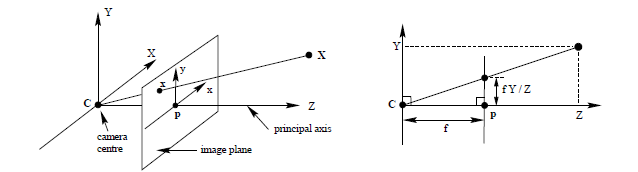
\includegraphics[width=.8\linewidth]{images/pinhole HZ.png}
	\captionof{figure}{Lochkameramodell \cite{Jianzhong}}
	\label{fig:PinholeCamera}
\end{minipage}\\ \\




\subsection{Kameraparameter}

Was bedeutet nun Szenenrekonstruktion und Kamerakalibrierung eines Stereoaufbaus im Zusammenhang mit dem gerade vorgestellten Kameramodell. In Abblildung ??? ist ein Stereoaufbau aus zwei Lochkameramodellen dargestell. Jede Kamera besitz ein eigenes Kamerakoordinatensystem und eine eigene Bildebene, welche wiederrum ein eigenes Bildnebenkoordinatensystem besitzt. Des Weiteren ist ein Objektpunkt $M$ in Bezug auf ein Weltkoordinatensystem zu sehen. Die zwei Strahlen die jeweils von $M$ ausgehen, beschreiben die Projektion des 3D-Objektpunktes $m$ auf die Bildpunkte $m$ und $m'$ auf den jeweiligen Bildebenen. Diese Projektion funktioniert auch in die andere Richtung. Sind zwei zueinandern korresponiderende Bildpunkte auf den beiden Bildebenen gegeben, so kann jeweils ein Strahl durch die jeweiligen Projektionszentren $C$ und $C'$ und deren zugehörigen Bildebenenpunkte $m$ und $m'$ geschickt werden, welche sich dann in einem Punkt $M$ im Raum treffen. Diese umgekehrte Rekonstruktion eines Punktes  wird allgemein als Triangulation bezeichnet\cite{HZ}. Hier werden jetzt die Projektionsmatrizen $P$ und $P'$ eingeführt, welche die Projektion $M$ auf $m$ und $m'$ beschreiben mit $m = PM$ und $m' = P'M$ und genaus so auch anders herum gelten für die Rückprojektion von $m$ und $m'$ auf $M$\cite{CamerModels.,HZ}.\\


(Skizze zwei Lochkameramodelle für den Steroskopieaufbau, backprojecting of point)\\


Die Projektionsmatrizen $P$ und $P'$ bilden sich aus den extrinsischen und intrinsischen Kameraparametern. Bei den extrinsischen Kameraparametern, handelt es sich um die jeweilige Orientierung einer Kamera bezüglich eines Weltkoordinatensystems, was in einer $3\times 4$-Transformationsmatrix $R$ beschrieben ist. $R$ kann sowohl eine Rotation als auch eine Translation beinhalten. Die intrinsischen Kameraparameter werden in der sogenannten Kameramatrix $K$ ausgedrückt. In der Literatur findet man diese wie folgt definiert\cite{HZ}.

\begin{gather}
K=\begin{bmatrix}
\alpha_x&s&x_{0}\\
0&\alpha_y&y_{0}\\
0&0&1
\end{bmatrix}
\end{gather}\\

Im folgenden werden die Elemente der Kameramatri $K$ im einzelnen beschrieben. Wird nochmal von dem in Abblidung ??? beschriebenen simplen Kameramodell ausgegangen, so lässt sich ein Dreidimensionaler homogenisierter Punkt $M$ mit $M = [X Y Z 1]^T$ durch aufstellen einer Matrix in einen homogenen 2D-Bildebenenpunkt $m$ mit $m = [\zeta X \zeta Y 1]^T$ ausdrücken.

\begin{gather}
	\begin{bmatrix}
	X\\Y\\Z\\1
	\end{bmatrix} \mapsto
	\begin{pmatrix}
	\zeta X\\ \zeta Y\\ Z
	\end{pmatrix}
	=
	\begin{bmatrix}
	\zeta&0&0&0\\
	0&\zeta&0&0\\
	0&0&1&0
	\end{bmatrix}
	\cdot
	\begin{bmatrix}
	X\\Y\\Z\\1
	\end{bmatrix}
	=
	\begin{pmatrix}
	\zeta \frac{X}{Z}\\ \zeta \frac{Y}{Z}\\1
	\end{pmatrix}
\end{gather}\\



\begin{minipage}{\linewidth}
	\centering
	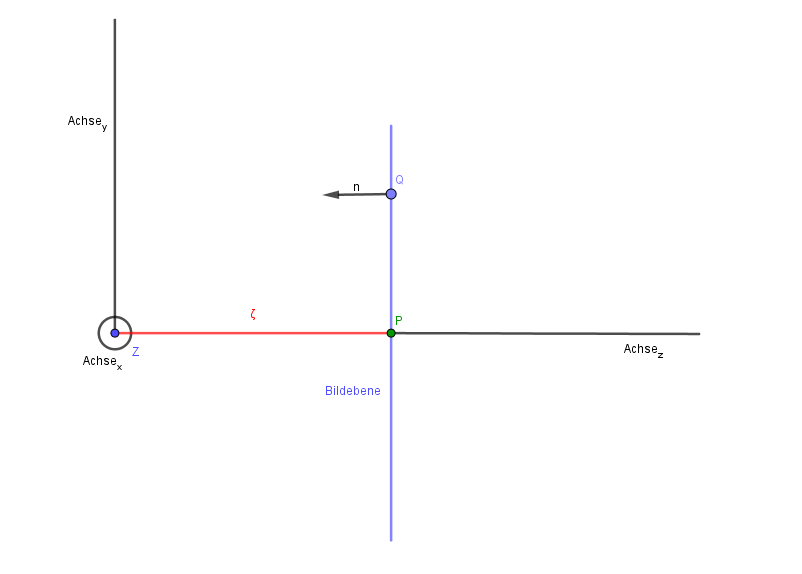
\includegraphics[width=1.\linewidth]{images/ZetaHerleitung.png}
	\captionof{figure}{In blau ist die Bildebene dargestellt auf ihr befinden sich die Punkte $Q$ und $P$. $P$ steht in dieser Abbildung für den Hauptpunkt. $Z$ liegt nicht auf der Ebene, Das Projetionszentrum $C$ liegt hinter der Bildebene und somit auch hinter dem Sensor. $n$ ist die Normale der Bildebene}
	\label{fig:zetaErklaerung}
\end{minipage}\\

Wie in Abbildung \ref{fig:zetaErklaerung} ersichtlich kann $\zeta$, welche den Abstand des Projektionszentrums zur Bildebene beschreibt, durch folgende Gleichung geometrisch bestimmt werden.

\begin{gather}
\vec{p}+|\vec{QZ} \cdot \vec{n}|\vec{n} = \vec{Z}
\end{gather}

$Q$ beschreibt einen beliebigen Punkt auf der Bildebene.

\begin{gather}
\vec{QZ} \cdot \hat{n} = \zeta\\
\vec{p}= \vec{Z}\zeta \hat{n}
\end{gather}

Bestimmt man nun, dass die Hauptachse $= \hat{n}$ ist, kann daraus geschlossen werden, dass $\vec{p} = \vec{Z} - \zeta \hat{n}$

$\zeta$ gibt wie bereits erwähnt den Abstand des Projektionszentrums $C$ zum Hauptpunkt der Bildebene an. 
In der Literatur  wird $\zeta$ meist mit $f$ für \textit{focal length} dargestellt und die Bildebene auch \textit{Focal plane} genannt \cite{HZ}.\\

(erklären warum focal length eigentlich die falsche bezeichnung ist)\\

Um die Kameramatrix allgemeiner zu formulieren und die Bedeutung hinter $\zeta$ und dessen Zusammenhang mit dem in der Literatur benutzten $f$ genauer zu erläutern, wird die Kameramatrix der Photogrammetrie in Bezug auf ein Lochkameramodell hier noch einmal genauer betrachtet und mit dem hergeleiteten Modell verglichen\cite{HZ,Heipke}. Angenommen es gilt $\zeta = f$, dann gilt für die Projektion von Punkten das selbe wie in Gleichung 2.49 nur mit $f$ statt $\zeta$. 

\begin{gather}
\begin{bmatrix}
X\\Y\\Z\\1
\end{bmatrix} \mapsto
\begin{pmatrix}
f X\\ f Y\\ Z
\end{pmatrix}
=
\begin{bmatrix}
f&0&0&0\\
0&f&0&0\\
0&0&1&0
\end{bmatrix}
\cdot
\begin{bmatrix}
X\\Y\\Z\\1
\end{bmatrix}
=
\begin{pmatrix}
f \frac{X}{Z}\\ f \frac{Y}{Z}\\1
\end{pmatrix}
\end{gather}

Zum Vergleich dient die Definition im Buch von \textit{Hartley \& Zisserman}\cite{HZ}, welche der selbst hergeleiteten entspricht.


\begin{gather}
\begin{bmatrix}
X\\Y\\Z\\1
\end{bmatrix} \mapsto
\begin{pmatrix}
f X\\ f Y\\ Z
\end{pmatrix}
=
\begin{bmatrix}
f&0&0&0\\
0&f&0&0\\
0&0&1&0
\end{bmatrix}
\cdot
\begin{bmatrix}
X\\Y\\Z\\1
\end{bmatrix}
\end{gather}		


Die allgemeine Form der Kameramatrix bezogen auf das Lochkameramodell wird wie in Gleichung 2.1 gezeigt beschrieben. Anstelle von $f$ steht in der Kameramatrix aus Gleichung 2.1 $\alpha_x$ und $\alpha_y$. Die Werte welche $\alpha_x$ und $\alpha_y$ annehmen können, hängen von der geometrischen Form der Pixel des in der Kamera verbauten Sensors ab\cite{HZ,Photonik}.  $\alpha_x$ und $\alpha_y$ sind genau dann einheitlich, wenn die Form der verbauten Pixel, ebenfalls einheitlich quadratisch ist. Die Einheiten der x- und y- Achsen des Sensorkoordinatensystems sind einheitlich. $\alpha_x$ und $\alpha_y$ sind also genau dann ungleich, wenn die auf dem Sensor verbauten Pixel beispielsweise rechteckig oder die geometrische Form eines Parallelogramms besitzen\cite{HZ}. Im Stereoaufbau dieser Arbeit, wurden Kameras mit CMOS-Chips mit quadratischen Pixeln verwendet, weshalb $\alpha_x$ und $\alpha_y$ einheitlich sein werden. $\alpha_x$ und $\alpha_y$ entstehen aus der Multiplikation der Werte für $\zeta_x$ und $\zeta_y$ beziehungsweise  $f_x$ und $f_y$ mit einem jeweiligen Skalierungswert $m_x$ und $m_y$. Sind die Pixel nicht quadratisch, wird auf die Werte $f_x$ und $f_y$ jeweils eine Skalierung $m_x$ und $m_y$ drauf multipliziert so dass  $\alpha_x = f_x \cdot m_x$ und $\alpha_y = f_y \cdot m_y$ entspricht\cite{HZ}. Die Matrixeinträge,$x_{0}$ und $y_{0}$, bilden einen Translationsvektor. Sie beinhalten die Position des Hauptpunkts auf der Bildebene. $x_{0}$ und $y_{0}$ sind definiert als $x_{0} = p_x \cdot m_x$ und $x_{0} = p_y \cdot m_y$. Der Matrixeintrag $s$ wird dem sogenannten \textit{skew-Faktor} zugeordnet, welcher nur dann zum Einsatz kommt, sollte die optische Achse nicht orthogonal auf den Bildsensor auftreffen. Sprich wenn der Chip geneigt in der Kamera montiert wurde\cite{HZ}. Die komplette Projektionsmatrix $P=KR$\cite{HZ} besteht aus der Matrixmultiplikation der hergeleiteten Transformationsmatrix $R$ welche die externen Kamerparameter repräsentiert und der Kameramatrix $K$, welche die internen Kameraparameter repräsentiert\cite{HZ,ZZGXr}.


